\subsection{Implementation hpcasia}\label{Implementation}

\begin{figure}
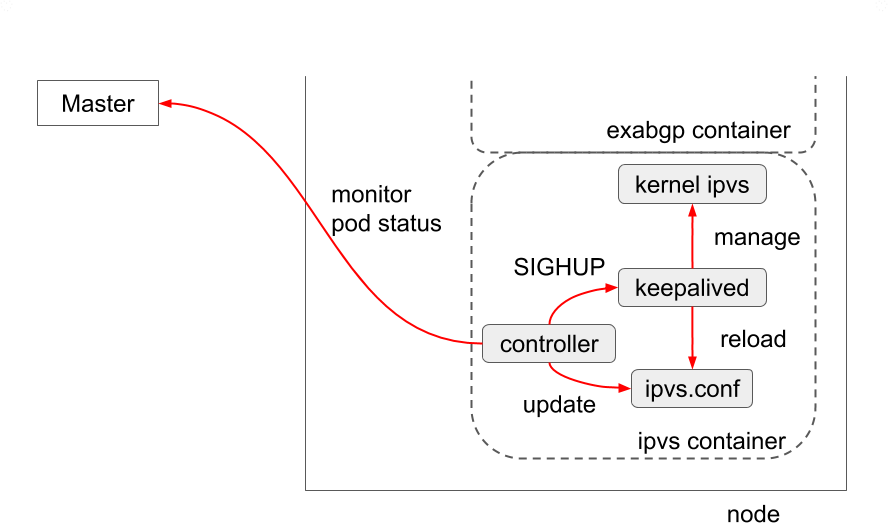
\includegraphics[width=\columnwidth]{Figs/ipvs-ingress-schem}
\caption{Implementation}
\label{fig:IPVS-ingress-schem}
\end{figure}

The proposed load balancer needs to dynamically reconfigure the IPVS balancing rules whenever {\em pods} are created/deleted. 
Figure~\ref{fig:IPVS-ingress-schem} is a schematic diagram to show the dynamic reconfiguration of the IPVS rules.
The right part of the figure shows the enlarged view of one of the nodes where the load balancer pod(LB2) is deployed.
Two daemon programs, controller and keepalived, run in the container inside the LB2 pod are illustrated.
The keepalived manages Linux kernel's IPVS rules depending on the ipvs.conf configuration file.
It is also capable of health-checking the liveliness of {\em real server}, 
which is represented as a combination of the IP addresses and port numbers of the target {\em pods}. 
If the health check to a {\em real server} fails, keepalived will remove that {\em real server} from the IPVS rules.

The controller monitors information concerning the running {\em pods} of a service 
in the Kubernetes cluster by consulting the apiserver running on the master.
Whenever {\em pods} are created or deleted, the controller will automatically regenerate an appropriate ipvs.conf 
and issue SIGHUP to keepalived.
Then, keepalived will reload the ipvs.conf and modify the kernel's IPVS rules accordingly.
The actual controller\cite{ktaka_ccmp_2017_826894} is implemented using the Kubernetes ingress controller\cite{K8sIngress2017} framework. 
By importing existing Golang package, \enquote{k8s.io/ingress /core/pkg/ingress}, we could simplify the implementation, e.g. 
120 lines of code.  

%In this way, the IPVS's balancing rules inside Linux kernel are maintained so that it can distribute the incoming traffic only to the living pods.

Configurations for capabilities were needed in the implementation: adding the CAP\_SYS\_MODULE capability 
to the container to allow the kernel to load required kernel modules inside a container, 
and adding CAP\_NET\_ADMIN capability to the container to allow keepalived to manipulate the kernel's IPVS rules. 
For the former case, we also needed to mount the \enquote{/lib/module} of the node's file system on the container's file system.

\begin{figure}
\begin{minipage}{0.7\columnwidth}
\begin{verbatim}
virtual_server fwmark 1 {
  delay_loop 5
  lb_algo lc
  lb_kind NAT
  protocol TCP
  real_server 172.16.21.2 80 {
    uthreshold 20000
    TCP_CHECK {
      connect_timeout 5
      connect_port 80
    }
  }
  real_server 172.16.80.2 80 {
    uthreshold 20000
    TCP_CHECK {
      connect_timeout 5
      connect_port 80
    }
  }
}
\end{verbatim}
\end{minipage}
\caption{An example of ipvs.conf}
\label{fig:ipvs.conf}
\end{figure}

\begin{figure}
\begin{minipage}{\columnwidth}
\small
\begin{verbatim}
# kubectl exec -it IPVS-controller-4117154712-kv633 -- IPVSadm -L
IP Virtual Server version 1.2.1 (size=4096)
Prot LocalAddress:Port Scheduler Flags
  -> RemoteAddress:Port Forward Weight ActiveConn InActConn
FWM  1 lc
  -> 172.16.21.2:80      Masq    1      0          0         
  -> 172.16.80.2:80      Masq    1      0          0
\end{verbatim}
\end{minipage}
\caption{Example of IPVS balancing rules}
\label{fig:IPVS rule}
\end{figure}


Figure~\ref{fig:ipvs.conf} and Figure~\ref{fig:IPVS rule} show an example of an ipvs.conf file 
generated by the controller and the corresponding IPVS load balancing rules, respectively.
Here, we can see that the packet with {\tt fwmark=1}\cite{BertHubert2002} is distributed 
to {\tt 172.16.21.2:80} and {\tt 172.16.80.2:80} 
using the masquerade mode(Masq) and 
the least connection(lc)\cite{Zhang2000} balancing algorithm.

